\begin{tikzpicture}
	\node (outer) at (3.5,1.2) {\makecell{\small Outer\\Race}};
	\node (inner) at (3.5,0) {\makecell{\small Inner\\Race}};
	\node (ball) at (3.5,-1.2) {\makecell{\small Ball\\(in cage)}};
	
	\node (outer2) at (1.3,1.2) {};
	\node (inner2) at (.3,0) {};
	\node (ball2) at (-.5,-1.2) {};

	\node[inner sep=0] (image) at (0,0) {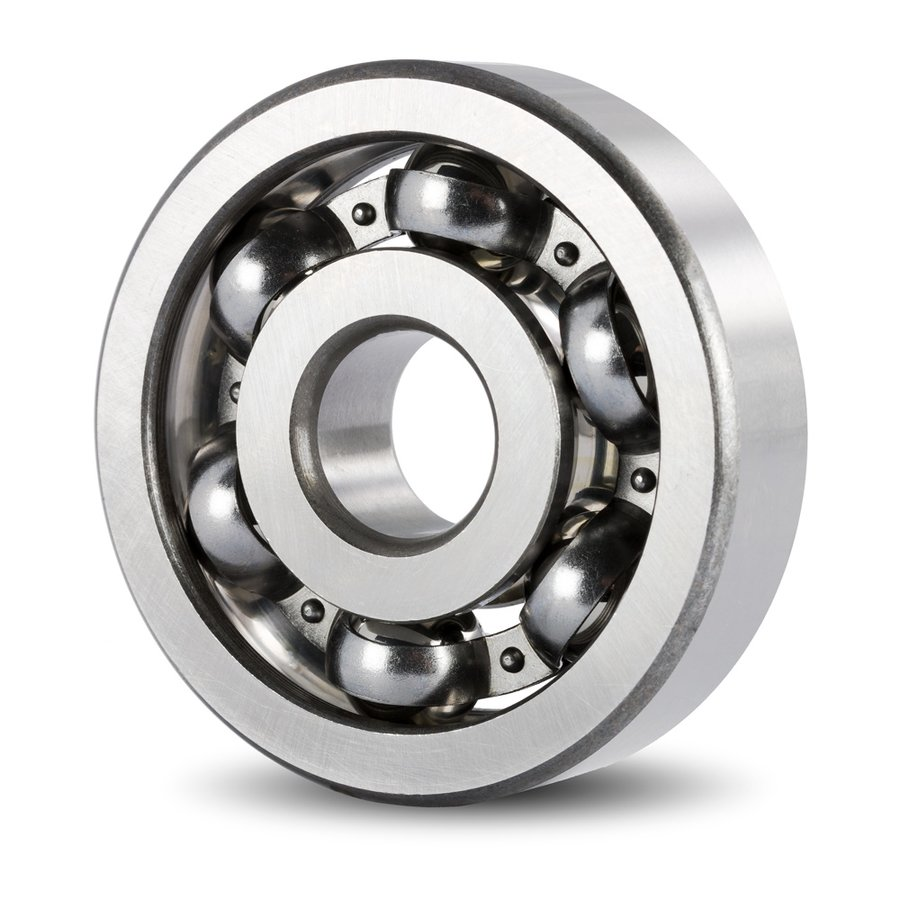
\includegraphics[width=0.35\textwidth]{figures/skf.jpg}};

	\draw [|->,  thick, red] (outer.west) -- (outer2);
	\draw [|->,  thick, red] (ball) -- (ball2);
	\draw [|->,  thick, red] (inner) -- (inner2);
\end{tikzpicture}